\documentclass[a4paper,11pt,titlepage]{article}
\usepackage[T1]{fontenc}
\usepackage[utf8]{inputenc}
\usepackage[frenchb]{babel}
\usepackage{lmodern}
\usepackage[final,expansion=true,protrusion=true]{microtype}
\usepackage[top=25mm,bottom=25mm,left=20mm,right=20mm]{geometry}
\usepackage[hidelinks,unicode]{hyperref}
\usepackage{fancyhdr}
\usepackage{graphicx}

\author{Laurent Girod \href{mailto:laurent.girod@heig-vd.ch}{\texttt{<laurent.girod@heig-vd.ch>}}\\
	Karel Ngueukam Djeuda Wilfried \href{wilfried.ngueukamdjeuda@heig-vd.ch}{\texttt{<wilfried.ngueukamdjeuda@heig-vd.ch>}}\\
	Rick Wertenbroek \href{mailto:rick.wertenbroek@heig-vd.ch}{\texttt{<rick.wertenbroek@heig-vd.ch>}}\\
	Cyrill Zundler \href{mailto:cyrill.zundler@heig-vd.ch}{\texttt{<cyrill.zundler@heig-vd.ch>}}
}
\date{\today}
\title{BDR\\Laboratoire no. 5}

\lhead{Laurent Girod\quad{}Karel Ngueukam Djeuda Wilfried\\Rick Wertenbroek\quad{}Cyrill Zundler}
\chead{RES---lab. 05}
\rhead{\today}
\lfoot{}
\cfoot{\thepage}
\rfoot{}

\pagestyle{fancy}

\setcounter{secnumdepth}{2}
\setcounter{tocdepth}{4}

\begin{document}
\maketitle
\tableofcontents
\newpage

\section[Introduction]{Introduction\protect\footnote{Fortement inspiré de \texttt{README.md} fourni dans le cadre de ce laboratoire.}}
Le but principal de ce laboratoire est d'apprendre à mettre en place une architecture web, et de se familiariser avec
des différents composants, tels que les serveurs HTTP, les \emph{load balancers} ou les \emph{reverse proxies}.

Il est également nécessaire de mettre en place un système de découverte automatique de services permettant de ``voire''
si un serveur HTTP est apparu ou a disparu de l'infrastructure et a réagir a ces changement en modifiant
automatiquement la configuration du \emph{load balancer}.

Le tout est fait dans un environnement virtualisé en utilisant \emph{Vagrant} et \emph{Docker}. 

\section{Architecture du système}
Après nous être concertés pour déterminer le genre de services offerts par l'architecture web, nous nous sommes entendus
pour créer un distributeur de citations générées par le programme UNIX \emph{fortune}.
\begin{figure}[h!]
	\centering
	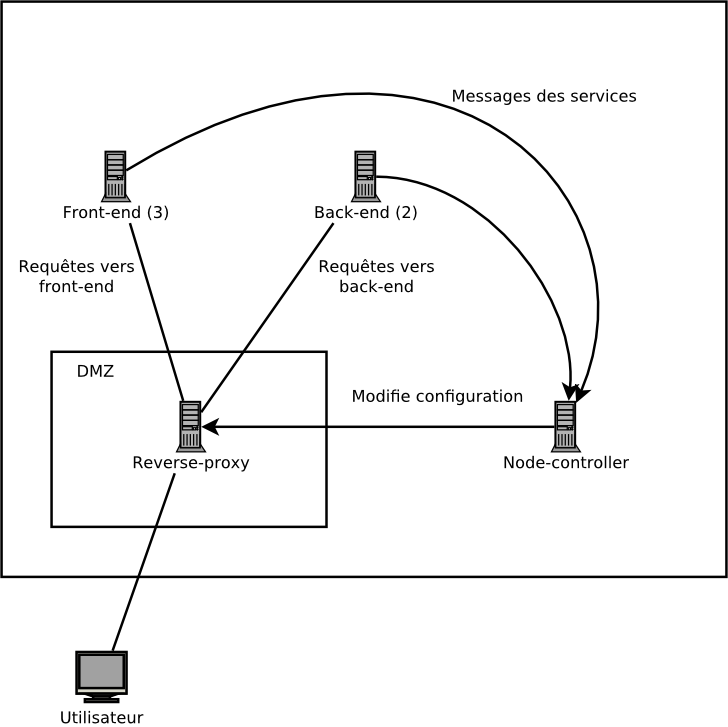
\includegraphics[scale=0.5]{schema.png}
	\caption{Architecture du système}
\end{figure}

\subsection{Détails des container}
\subsubsection{\emph{Back-end}}
Le \emph{back-end} est un serveur HTTP répondant à chaque requête par un JSON contenant une citation et
l'adresse IP du back-end selon le motif suivant:
\begin{center}
\texttt{\{"quote":"<citation>","ip":"<IP du backend>"\}}
\end{center}
L'utilité de fournir l'adresse IP est de donner une preuve au testeur que le \emph{load-balancer} (décrit ci-après)
fonctionne correctement.

Afin d'avoir un système le plus léger possible, et qui soit aisé à implémenter, le \emph{back-end} à été réalisé en
javascript avec \emph{Node.js}.

En parallèle, le \emph{back-end} possède un \emph{Heartbeat generator}, un programme en javascript envoyant en continu
toutes les 10 secondes un message en UDP sur un port définit, sur l'adresse IP multicast définie \texttt{224.1.1.1}.
Ce message JSON contient les 2 champs suivants:

\begin{itemize}
	\item le type du client ( backend ou fronten ) 
	\item l'ID du container \emph{Docker}
\end{itemize}

\subsubsection{\emph{Front-end}}
Le \emph{front-end} est un serveur HTTP répondant à chaque requête par un page HTML contenant un javascript permettant
de faire une requête pour récupérer une citation. Cette requête sera redirigée vers le back-end par le
\emph{reverse-proxy}. Afin de fournir une preuve au testeur que le \emph{load-balancer} fonctionne correctement, la page
HTML générée contient l'adresse IP du \emph{front-end}.

Pour les même raisons que pour le \emph{back-end}, le \emph{front-end} à été réalisé en javascript avec \emph{Node.js}.

De la même manière que le \emph{back-end}, le \emph{front-end} possède lui aussi un \emph{heartbeat generator} envoyant
des messages en continu sur l'adresse multicast \texttt{224.1.1.1} et sur un port définit.

\subsubsection{\emph{Node controller}}
Le \emph{node controller} (server) écoute sur un port et attend des paquet entrant contenant 2 champs:

\begin{itemize}
	\item le type 
	\item l'ID du container \emph{Docker}
\end{itemize}

Le contrôleur contient une structure de donnée \texttt{client} et un tableau de client \texttt{clients[]}.

La structure de donnée \texttt{client} contient simplement des variable\footnote{voir code source}: \texttt{ip},
\texttt{id}, \texttt{type}, \texttt{date}\footnote{\texttt{DATE} = chiffre représentant le nombre de millisecondes
écoulées depuis l'epoch.}, \ldots

À l'arrivée d'un message pas un client le serveur crée un client avec la structure décrite ci-dessus.

Si l'adresse IP du client qui vient d'envoyer le message n'est pas contenu dans le tableau de clients que contient le serveur, 
le \emph{node controller} ajoute le client précédemment créé au tableau de clients, met à jour le fichier de configuration
d'\emph{Apache} et redémarre le \emph{reverse proxy}. Sinon, si l'adresse IP du client est déjà contenue dans le tableau, le
\emph{node controller} ne fait que mettre à jour le timestamp du client en question, puis supprime le client précédemment créé. 

En parallèle de ceci, Le serveur parcoure toutes les 5 seconde le tableau de client et vérifie le \emph{timestamp} de chaque
client. Si le temps écoulé depuis son arrivée dépasse 10 secondes, le \emph{node controler} retire le client de la liste et
met à jour le fichier de configuration d'\emph{Apache} et redémarre le \emph{reverse proxy}, sinon ne fait rien.

\subsubsection{\emph{Reverse proxy et load balancer}}
Nous avons choisi d'implémenter ce point grâce au service \emph{httpd} (\emph{Apache 2}).

Le \emph{reverse proxy} est le seul point d'entrée extérieur à notre architecture. En effet il sert à masquer le fait qu'il y
aie plusieurs machines derrière une adresse, il se chargera de transmettre les différentes requêtes au bon endroit et de
retourner les réponses. Il fait en même temps la distribution du travail (\emph{load balancer}) lorsqu'il a plusieurs
possibilités vers qui envoyer une requête (parce qu'on a plusieurs machines qui sont capables de faire la même chose,
plusieurs \emph{front-end} et \emph{back-end}) il va choisir de les distribuer équitablement afin de partager le travail.
Nous avons choisi ici d'implémenter une méthode ``Round-Robin''. La communication avec le \emph{front-end} est en
\emph{sticky session} avec un cookie qui permet de spécifier la route (donc quel \emph{front-end}) comme ça si un client a
commencé à communiquer avec un \emph{front-end} il va continuer avec ce \emph{front-end} tant qu'il donne le cookie, si un
nouveau client arrive (sans cookie donc) le \emph{load balancer} va le rediriger au prochain \emph{front-end} comme indiqué
par notre police ``Round-Robin''.

Le fichier de configuration du \emph{reverse proxy} ---\emph{load balancer} est généré par le \emph{node controller} et est
mis à jour à chaque changement dans les services disponibles (nouveau \emph{front-end} ou \emph{back-end} ou bien si un
\emph{front-end} ou \emph{back-end} n'est plus disponible). Pour rendre effectif la modification nous relançons la machine
depuis le \emph{node controller} (qui a les privilèges) avec \emph{Dockerode}, dans le fichier de configuration de
\emph{httpd} il est spécifié de charger notre fichier de configuration spécifique qui est partagé entre le \emph{node
controller} et cette machine.

Note: La route pour la \emph{sticky session} est l'ID unique du container vers qui la route pointe, ceci nous garantit que si
la machine tombe et se relance la route sera conservée, si on utilisais des entier (1, 2, 3, \ldots) si la machine 2 tombe et
que la machine 3 prends la place du 2 la route 2 renverrait vers une autre machine qu'auparavant. Avec les ID uniques une
route ne pointera que vers une seule machine et toujours la même.

\subsection{Protocoles de communications utilisés}
Tous les échanges effectués entre les \emph{front-end}s, les \emph{back-end}s et le \emph{node controller} sont effectués par
UDP et sont des JSONs.

\section{Strategie de validation}
\subsection{Test du \emph{load balancer}}
Afin de tester que notre implémentation soit correcte, un web browser (Google Chrome) a été utilisé pour ouvrir la page web,
qui affiche aussi bien l'adresse IP du \emph{font-end} que celle du \emph{back-end}. Lorsque la quote était renouvellée en
appuyant sur le bouton de la page web pour renouveller les quotes, l'adresse IP du \emph{back-end} était effectivement modifiée.
Par contre, si la page était rechargée, le \emph{front-end} était le même. Ce qui est normal, le cookie est conservé. En
utilisant le mode de navigation privée de Chrome, qui ne conserve pas les cookies, et n'utilise pas de cache, l'adresse IP du
\emph{front-end} change avec un rechargement de la page. Le \emph{load balancer} fonctionne donc correctement.

\subsection{Test du \emph{node controller}}
Afin de tester si le système détecte l'apparition ou la disparition d'un node, un container \emph{Docker} est supprimé, dans
les quelques secondes suivantes, la configuration du \emph{reverse proxy} est modifié pour prendre en compte la disparition du
n\oe{}ud. Ensuite un nouveau container \emph{Docker} est créé. À nouveau, la configuration est modifiée pour prendre en compte
ces changements. 

\subsection{Marche à suivre pour valider l'architecture}
\subsubsection{Mise en place}
\begin{enumerate}
	\item Lancer Vagrant dans le repertoire ou se trouve le fichier \texttt{Vagrantfile}.\\
		\texttt{\$ vagrant up}
	\item Se logger dans vagrant.\\
		\texttt{\$ vagrant ssh}
	\item Créer les images \emph{Docker} à l'aide des scripts fournis.\\
		\texttt{\$ cd /vagrant/backend}\\
		\texttt{\$ ./createDockerImage.sh}\\
		\texttt{\$ cd /vagrant/frontend}\\
		\texttt{\$ ./createDockerImage.sh}\\
		\texttt{\$ cd /vagrant/node-controller}\\
		\texttt{\$ ./createDockerImage.sh}\\
		\texttt{\$ cd /vagrant/reverse-proxy-lb}\\
		\texttt{\$ ./createDockerImage.sh}
	\item (facultatif) Si on veut visulaiser les container \emph{Docker} avec une interface graphique, on peut aussi construire
		l'image \emph{DockerUI}\\
		\texttt{\$ cd /vagrant/dockerUI}\\
		\texttt{\$ ./createDockerImage.sh}
	\item Lancer les container \emph{Docker} à l'aide des scripts fournis. (Notons qu'il faut fournir un nom pour les back-ends et front-ends)\\
		\texttt{\$ cd /vagrant/backend}\\
		\texttt{\$ ./startContainers.sh backend1}\\
		\texttt{\$ ./startContainers.sh backend2}\\
		\texttt{\$ cd /vagrant/frontend}\\
		\texttt{\$ ./startContainers.sh frontend1}\\
		\texttt{\$ ./startContainers.sh frontend2}\\
		\texttt{\$ ./startContainers.sh frontend3}\\
		\texttt{\$ cd /vagrant/node-controller}\\
		\texttt{\$ ./startContainers.sh}\\
		\texttt{\$ cd /vagrant/reverse-proxy-lb}\\
		\texttt{\$ ./startContainers.sh}
	\item (facultatif) Si on veut utiliser DockerUI, il faut aussi lancer un container.\\
		\texttt{\$ cd /vagrant/dockerUI}\\
		\texttt{\$ ./startContainers.sh}
\end{enumerate}

\subsubsection{Test du \emph{back-end}, du \emph{front-end}, et du \emph{reverse proxy}}
\begin{enumerate}
	\item Lancer un navigateur web (par exemple Google Chrome) et entrer l'url \texttt{192.168.42.42} en utilisant le port standard (80).
Nous pouvons voire l'adresse IP du front-end et du back-end.
\end{enumerate}
\begin{center}
	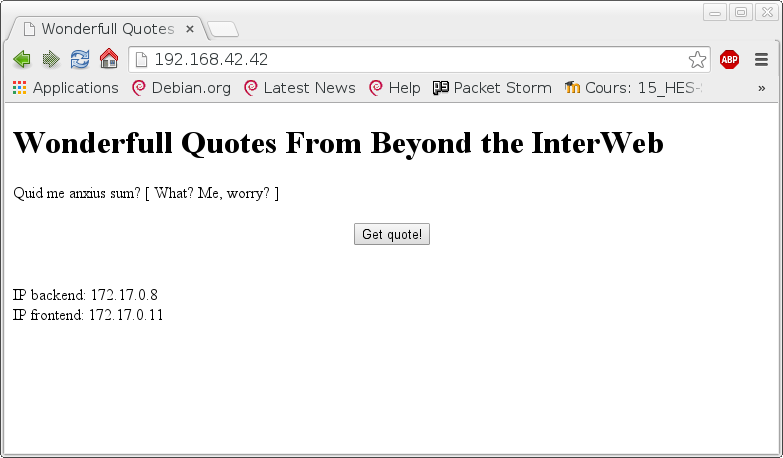
\includegraphics[scale=0.5]{test1.png}
\end{center}

À présent nous sommes sûr que le \emph{back-end}, le \emph{front-end}, et le \emph{reverse proxy} fonctionnent.

\subsubsection{Test du load balancer}
\begin{enumerate}
	\item Appuyer plusieurs fois sur le boutton ``\emph{Get quote!}''. Nous pouvons voire que l'adresse IP du front-end reste fixe, mais que celle du back-end change.
	\item Recharger plusieurs fois la page après avoir éliminé les cookies du navigateur. Nous observons que l'adresse IP du front-end est aussi modifiée.
\end{enumerate}
\begin{center}
\begin{tabular}{cc}
	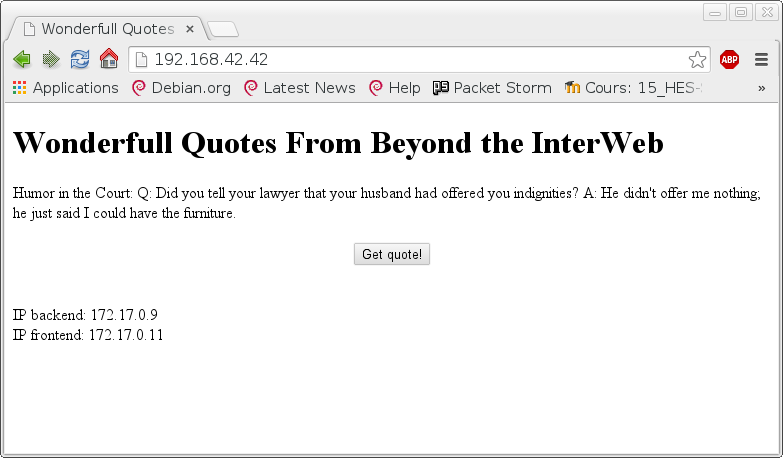
\includegraphics[scale=0.3]{test2.png} & 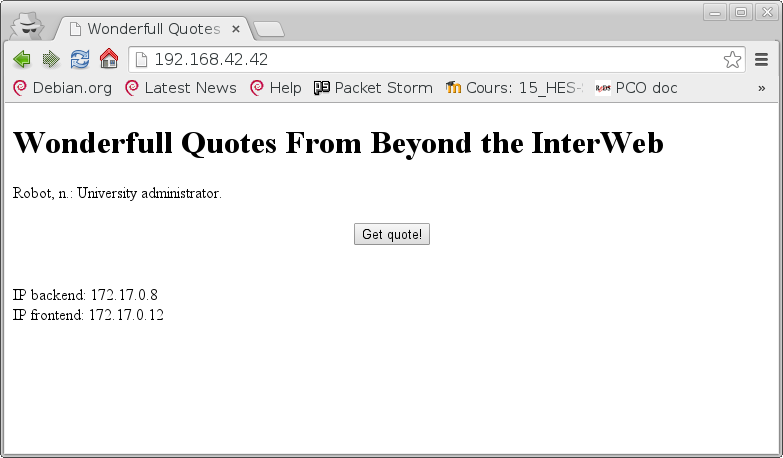
\includegraphics[scale=0.3]{test3.png} \\
	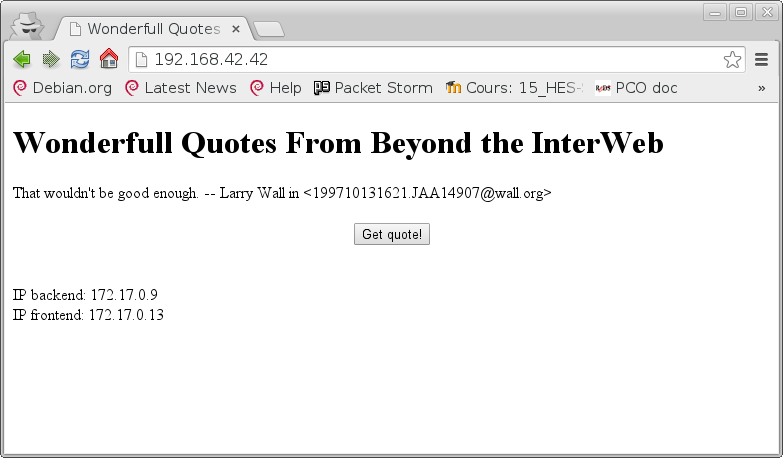
\includegraphics[scale=0.3]{test4.png} & 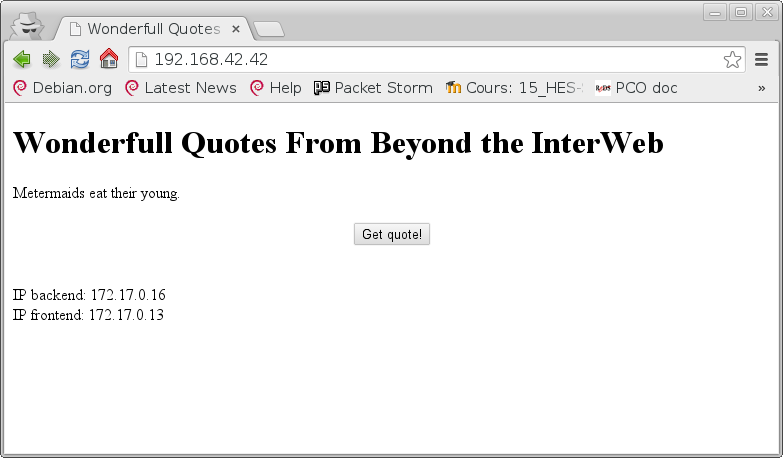
\includegraphics[scale=0.3]{test5.png} \\
\end{tabular}
\end{center}

À présent nous sommes sûr que le \emph{load balancer} fonctionne.

\subsubsection{Test du node balancer}
\begin{enumerate}
	\item Nous démarrons des nouveaux \emph{back-end}s ou des nouveaux \emph{front-end}s.
Après quelques secondes, ils sont trouvés par le \emph{node balancer}, et peuvent être utilisés.
	\item Nous supprimons des \emph{back-end}s ou des \emph{front-end}s
Après quelques secondes, le \emph{node balancer} a reconfiguré le \emph{load balancer} pour prendre en compte le nouvel état du système.
Il est possible de lire ce fichier, qui se trouve dans le répertoire ``\texttt{shared\_volume}'', et est nommé ``\texttt{httpd-vhosts.conf}'',
et de trouver uniquement les containers \emph{Docker} disponibles.
\end{enumerate}

À présent nous sommes sûr que le \emph{node controller} fonctionne.

\section{Conclusions}
À la fin de ce laboratoire, nous avons obtenu un système fonctionnel, et se comportant de manière idoine, et fidèle aux
objectifs fixés. Nous avons également appris de manière concrète le fonctionnement d'une architecture web. Nous pouvons
donc en conclure que ce laboratoire est un succès.

\end{document}
